
% Default to the notebook output style

    


% Inherit from the specified cell style.




    
\documentclass[11pt]{article}

    
    
    \usepackage[T1]{fontenc}
    % Nicer default font (+ math font) than Computer Modern for most use cases
    \usepackage{mathpazo}

    % Basic figure setup, for now with no caption control since it's done
    % automatically by Pandoc (which extracts ![](path) syntax from Markdown).
    \usepackage{graphicx}
    % We will generate all images so they have a width \maxwidth. This means
    % that they will get their normal width if they fit onto the page, but
    % are scaled down if they would overflow the margins.
    \makeatletter
    \def\maxwidth{\ifdim\Gin@nat@width>\linewidth\linewidth
    \else\Gin@nat@width\fi}
    \makeatother
    \let\Oldincludegraphics\includegraphics
    % Set max figure width to be 80% of text width, for now hardcoded.
    \renewcommand{\includegraphics}[1]{\Oldincludegraphics[width=.8\maxwidth]{#1}}
    % Ensure that by default, figures have no caption (until we provide a
    % proper Figure object with a Caption API and a way to capture that
    % in the conversion process - todo).
    \usepackage{caption}
    \DeclareCaptionLabelFormat{nolabel}{}
    \captionsetup{labelformat=nolabel}

    \usepackage{adjustbox} % Used to constrain images to a maximum size 
    \usepackage{xcolor} % Allow colors to be defined
    \usepackage{enumerate} % Needed for markdown enumerations to work
    \usepackage{geometry} % Used to adjust the document margins
    \usepackage{amsmath} % Equations
    \usepackage{amssymb} % Equations
    \usepackage{textcomp} % defines textquotesingle
    % Hack from http://tex.stackexchange.com/a/47451/13684:
    \AtBeginDocument{%
        \def\PYZsq{\textquotesingle}% Upright quotes in Pygmentized code
    }
    \usepackage{upquote} % Upright quotes for verbatim code
    \usepackage{eurosym} % defines \euro
    \usepackage[mathletters]{ucs} % Extended unicode (utf-8) support
    \usepackage[utf8x]{inputenc} % Allow utf-8 characters in the tex document
    \usepackage{fancyvrb} % verbatim replacement that allows latex
    \usepackage{grffile} % extends the file name processing of package graphics 
                         % to support a larger range 
    % The hyperref package gives us a pdf with properly built
    % internal navigation ('pdf bookmarks' for the table of contents,
    % internal cross-reference links, web links for URLs, etc.)
    \usepackage{hyperref}
    \usepackage{longtable} % longtable support required by pandoc >1.10
    \usepackage{booktabs}  % table support for pandoc > 1.12.2
    \usepackage[inline]{enumitem} % IRkernel/repr support (it uses the enumerate* environment)
    \usepackage[normalem]{ulem} % ulem is needed to support strikethroughs (\sout)
                                % normalem makes italics be italics, not underlines
    

    
    
    % Colors for the hyperref package
    \definecolor{urlcolor}{rgb}{0,.145,.698}
    \definecolor{linkcolor}{rgb}{.71,0.21,0.01}
    \definecolor{citecolor}{rgb}{.12,.54,.11}

    % ANSI colors
    \definecolor{ansi-black}{HTML}{3E424D}
    \definecolor{ansi-black-intense}{HTML}{282C36}
    \definecolor{ansi-red}{HTML}{E75C58}
    \definecolor{ansi-red-intense}{HTML}{B22B31}
    \definecolor{ansi-green}{HTML}{00A250}
    \definecolor{ansi-green-intense}{HTML}{007427}
    \definecolor{ansi-yellow}{HTML}{DDB62B}
    \definecolor{ansi-yellow-intense}{HTML}{B27D12}
    \definecolor{ansi-blue}{HTML}{208FFB}
    \definecolor{ansi-blue-intense}{HTML}{0065CA}
    \definecolor{ansi-magenta}{HTML}{D160C4}
    \definecolor{ansi-magenta-intense}{HTML}{A03196}
    \definecolor{ansi-cyan}{HTML}{60C6C8}
    \definecolor{ansi-cyan-intense}{HTML}{258F8F}
    \definecolor{ansi-white}{HTML}{C5C1B4}
    \definecolor{ansi-white-intense}{HTML}{A1A6B2}

    % commands and environments needed by pandoc snippets
    % extracted from the output of `pandoc -s`
    \providecommand{\tightlist}{%
      \setlength{\itemsep}{0pt}\setlength{\parskip}{0pt}}
    \DefineVerbatimEnvironment{Highlighting}{Verbatim}{commandchars=\\\{\}}
    % Add ',fontsize=\small' for more characters per line
    \newenvironment{Shaded}{}{}
    \newcommand{\KeywordTok}[1]{\textcolor[rgb]{0.00,0.44,0.13}{\textbf{{#1}}}}
    \newcommand{\DataTypeTok}[1]{\textcolor[rgb]{0.56,0.13,0.00}{{#1}}}
    \newcommand{\DecValTok}[1]{\textcolor[rgb]{0.25,0.63,0.44}{{#1}}}
    \newcommand{\BaseNTok}[1]{\textcolor[rgb]{0.25,0.63,0.44}{{#1}}}
    \newcommand{\FloatTok}[1]{\textcolor[rgb]{0.25,0.63,0.44}{{#1}}}
    \newcommand{\CharTok}[1]{\textcolor[rgb]{0.25,0.44,0.63}{{#1}}}
    \newcommand{\StringTok}[1]{\textcolor[rgb]{0.25,0.44,0.63}{{#1}}}
    \newcommand{\CommentTok}[1]{\textcolor[rgb]{0.38,0.63,0.69}{\textit{{#1}}}}
    \newcommand{\OtherTok}[1]{\textcolor[rgb]{0.00,0.44,0.13}{{#1}}}
    \newcommand{\AlertTok}[1]{\textcolor[rgb]{1.00,0.00,0.00}{\textbf{{#1}}}}
    \newcommand{\FunctionTok}[1]{\textcolor[rgb]{0.02,0.16,0.49}{{#1}}}
    \newcommand{\RegionMarkerTok}[1]{{#1}}
    \newcommand{\ErrorTok}[1]{\textcolor[rgb]{1.00,0.00,0.00}{\textbf{{#1}}}}
    \newcommand{\NormalTok}[1]{{#1}}
    
    % Additional commands for more recent versions of Pandoc
    \newcommand{\ConstantTok}[1]{\textcolor[rgb]{0.53,0.00,0.00}{{#1}}}
    \newcommand{\SpecialCharTok}[1]{\textcolor[rgb]{0.25,0.44,0.63}{{#1}}}
    \newcommand{\VerbatimStringTok}[1]{\textcolor[rgb]{0.25,0.44,0.63}{{#1}}}
    \newcommand{\SpecialStringTok}[1]{\textcolor[rgb]{0.73,0.40,0.53}{{#1}}}
    \newcommand{\ImportTok}[1]{{#1}}
    \newcommand{\DocumentationTok}[1]{\textcolor[rgb]{0.73,0.13,0.13}{\textit{{#1}}}}
    \newcommand{\AnnotationTok}[1]{\textcolor[rgb]{0.38,0.63,0.69}{\textbf{\textit{{#1}}}}}
    \newcommand{\CommentVarTok}[1]{\textcolor[rgb]{0.38,0.63,0.69}{\textbf{\textit{{#1}}}}}
    \newcommand{\VariableTok}[1]{\textcolor[rgb]{0.10,0.09,0.49}{{#1}}}
    \newcommand{\ControlFlowTok}[1]{\textcolor[rgb]{0.00,0.44,0.13}{\textbf{{#1}}}}
    \newcommand{\OperatorTok}[1]{\textcolor[rgb]{0.40,0.40,0.40}{{#1}}}
    \newcommand{\BuiltInTok}[1]{{#1}}
    \newcommand{\ExtensionTok}[1]{{#1}}
    \newcommand{\PreprocessorTok}[1]{\textcolor[rgb]{0.74,0.48,0.00}{{#1}}}
    \newcommand{\AttributeTok}[1]{\textcolor[rgb]{0.49,0.56,0.16}{{#1}}}
    \newcommand{\InformationTok}[1]{\textcolor[rgb]{0.38,0.63,0.69}{\textbf{\textit{{#1}}}}}
    \newcommand{\WarningTok}[1]{\textcolor[rgb]{0.38,0.63,0.69}{\textbf{\textit{{#1}}}}}
    
    
    % Define a nice break command that doesn't care if a line doesn't already
    % exist.
    \def\br{\hspace*{\fill} \\* }
    % Math Jax compatability definitions
    \def\gt{>}
    \def\lt{<}
    % Document parameters
    \title{Reliable Routing }
    
    
    

    % Pygments definitions
    
\makeatletter
\def\PY@reset{\let\PY@it=\relax \let\PY@bf=\relax%
    \let\PY@ul=\relax \let\PY@tc=\relax%
    \let\PY@bc=\relax \let\PY@ff=\relax}
\def\PY@tok#1{\csname PY@tok@#1\endcsname}
\def\PY@toks#1+{\ifx\relax#1\empty\else%
    \PY@tok{#1}\expandafter\PY@toks\fi}
\def\PY@do#1{\PY@bc{\PY@tc{\PY@ul{%
    \PY@it{\PY@bf{\PY@ff{#1}}}}}}}
\def\PY#1#2{\PY@reset\PY@toks#1+\relax+\PY@do{#2}}

\expandafter\def\csname PY@tok@w\endcsname{\def\PY@tc##1{\textcolor[rgb]{0.73,0.73,0.73}{##1}}}
\expandafter\def\csname PY@tok@c\endcsname{\let\PY@it=\textit\def\PY@tc##1{\textcolor[rgb]{0.25,0.50,0.50}{##1}}}
\expandafter\def\csname PY@tok@cp\endcsname{\def\PY@tc##1{\textcolor[rgb]{0.74,0.48,0.00}{##1}}}
\expandafter\def\csname PY@tok@k\endcsname{\let\PY@bf=\textbf\def\PY@tc##1{\textcolor[rgb]{0.00,0.50,0.00}{##1}}}
\expandafter\def\csname PY@tok@kp\endcsname{\def\PY@tc##1{\textcolor[rgb]{0.00,0.50,0.00}{##1}}}
\expandafter\def\csname PY@tok@kt\endcsname{\def\PY@tc##1{\textcolor[rgb]{0.69,0.00,0.25}{##1}}}
\expandafter\def\csname PY@tok@o\endcsname{\def\PY@tc##1{\textcolor[rgb]{0.40,0.40,0.40}{##1}}}
\expandafter\def\csname PY@tok@ow\endcsname{\let\PY@bf=\textbf\def\PY@tc##1{\textcolor[rgb]{0.67,0.13,1.00}{##1}}}
\expandafter\def\csname PY@tok@nb\endcsname{\def\PY@tc##1{\textcolor[rgb]{0.00,0.50,0.00}{##1}}}
\expandafter\def\csname PY@tok@nf\endcsname{\def\PY@tc##1{\textcolor[rgb]{0.00,0.00,1.00}{##1}}}
\expandafter\def\csname PY@tok@nc\endcsname{\let\PY@bf=\textbf\def\PY@tc##1{\textcolor[rgb]{0.00,0.00,1.00}{##1}}}
\expandafter\def\csname PY@tok@nn\endcsname{\let\PY@bf=\textbf\def\PY@tc##1{\textcolor[rgb]{0.00,0.00,1.00}{##1}}}
\expandafter\def\csname PY@tok@ne\endcsname{\let\PY@bf=\textbf\def\PY@tc##1{\textcolor[rgb]{0.82,0.25,0.23}{##1}}}
\expandafter\def\csname PY@tok@nv\endcsname{\def\PY@tc##1{\textcolor[rgb]{0.10,0.09,0.49}{##1}}}
\expandafter\def\csname PY@tok@no\endcsname{\def\PY@tc##1{\textcolor[rgb]{0.53,0.00,0.00}{##1}}}
\expandafter\def\csname PY@tok@nl\endcsname{\def\PY@tc##1{\textcolor[rgb]{0.63,0.63,0.00}{##1}}}
\expandafter\def\csname PY@tok@ni\endcsname{\let\PY@bf=\textbf\def\PY@tc##1{\textcolor[rgb]{0.60,0.60,0.60}{##1}}}
\expandafter\def\csname PY@tok@na\endcsname{\def\PY@tc##1{\textcolor[rgb]{0.49,0.56,0.16}{##1}}}
\expandafter\def\csname PY@tok@nt\endcsname{\let\PY@bf=\textbf\def\PY@tc##1{\textcolor[rgb]{0.00,0.50,0.00}{##1}}}
\expandafter\def\csname PY@tok@nd\endcsname{\def\PY@tc##1{\textcolor[rgb]{0.67,0.13,1.00}{##1}}}
\expandafter\def\csname PY@tok@s\endcsname{\def\PY@tc##1{\textcolor[rgb]{0.73,0.13,0.13}{##1}}}
\expandafter\def\csname PY@tok@sd\endcsname{\let\PY@it=\textit\def\PY@tc##1{\textcolor[rgb]{0.73,0.13,0.13}{##1}}}
\expandafter\def\csname PY@tok@si\endcsname{\let\PY@bf=\textbf\def\PY@tc##1{\textcolor[rgb]{0.73,0.40,0.53}{##1}}}
\expandafter\def\csname PY@tok@se\endcsname{\let\PY@bf=\textbf\def\PY@tc##1{\textcolor[rgb]{0.73,0.40,0.13}{##1}}}
\expandafter\def\csname PY@tok@sr\endcsname{\def\PY@tc##1{\textcolor[rgb]{0.73,0.40,0.53}{##1}}}
\expandafter\def\csname PY@tok@ss\endcsname{\def\PY@tc##1{\textcolor[rgb]{0.10,0.09,0.49}{##1}}}
\expandafter\def\csname PY@tok@sx\endcsname{\def\PY@tc##1{\textcolor[rgb]{0.00,0.50,0.00}{##1}}}
\expandafter\def\csname PY@tok@m\endcsname{\def\PY@tc##1{\textcolor[rgb]{0.40,0.40,0.40}{##1}}}
\expandafter\def\csname PY@tok@gh\endcsname{\let\PY@bf=\textbf\def\PY@tc##1{\textcolor[rgb]{0.00,0.00,0.50}{##1}}}
\expandafter\def\csname PY@tok@gu\endcsname{\let\PY@bf=\textbf\def\PY@tc##1{\textcolor[rgb]{0.50,0.00,0.50}{##1}}}
\expandafter\def\csname PY@tok@gd\endcsname{\def\PY@tc##1{\textcolor[rgb]{0.63,0.00,0.00}{##1}}}
\expandafter\def\csname PY@tok@gi\endcsname{\def\PY@tc##1{\textcolor[rgb]{0.00,0.63,0.00}{##1}}}
\expandafter\def\csname PY@tok@gr\endcsname{\def\PY@tc##1{\textcolor[rgb]{1.00,0.00,0.00}{##1}}}
\expandafter\def\csname PY@tok@ge\endcsname{\let\PY@it=\textit}
\expandafter\def\csname PY@tok@gs\endcsname{\let\PY@bf=\textbf}
\expandafter\def\csname PY@tok@gp\endcsname{\let\PY@bf=\textbf\def\PY@tc##1{\textcolor[rgb]{0.00,0.00,0.50}{##1}}}
\expandafter\def\csname PY@tok@go\endcsname{\def\PY@tc##1{\textcolor[rgb]{0.53,0.53,0.53}{##1}}}
\expandafter\def\csname PY@tok@gt\endcsname{\def\PY@tc##1{\textcolor[rgb]{0.00,0.27,0.87}{##1}}}
\expandafter\def\csname PY@tok@err\endcsname{\def\PY@bc##1{\setlength{\fboxsep}{0pt}\fcolorbox[rgb]{1.00,0.00,0.00}{1,1,1}{\strut ##1}}}
\expandafter\def\csname PY@tok@kc\endcsname{\let\PY@bf=\textbf\def\PY@tc##1{\textcolor[rgb]{0.00,0.50,0.00}{##1}}}
\expandafter\def\csname PY@tok@kd\endcsname{\let\PY@bf=\textbf\def\PY@tc##1{\textcolor[rgb]{0.00,0.50,0.00}{##1}}}
\expandafter\def\csname PY@tok@kn\endcsname{\let\PY@bf=\textbf\def\PY@tc##1{\textcolor[rgb]{0.00,0.50,0.00}{##1}}}
\expandafter\def\csname PY@tok@kr\endcsname{\let\PY@bf=\textbf\def\PY@tc##1{\textcolor[rgb]{0.00,0.50,0.00}{##1}}}
\expandafter\def\csname PY@tok@bp\endcsname{\def\PY@tc##1{\textcolor[rgb]{0.00,0.50,0.00}{##1}}}
\expandafter\def\csname PY@tok@fm\endcsname{\def\PY@tc##1{\textcolor[rgb]{0.00,0.00,1.00}{##1}}}
\expandafter\def\csname PY@tok@vc\endcsname{\def\PY@tc##1{\textcolor[rgb]{0.10,0.09,0.49}{##1}}}
\expandafter\def\csname PY@tok@vg\endcsname{\def\PY@tc##1{\textcolor[rgb]{0.10,0.09,0.49}{##1}}}
\expandafter\def\csname PY@tok@vi\endcsname{\def\PY@tc##1{\textcolor[rgb]{0.10,0.09,0.49}{##1}}}
\expandafter\def\csname PY@tok@vm\endcsname{\def\PY@tc##1{\textcolor[rgb]{0.10,0.09,0.49}{##1}}}
\expandafter\def\csname PY@tok@sa\endcsname{\def\PY@tc##1{\textcolor[rgb]{0.73,0.13,0.13}{##1}}}
\expandafter\def\csname PY@tok@sb\endcsname{\def\PY@tc##1{\textcolor[rgb]{0.73,0.13,0.13}{##1}}}
\expandafter\def\csname PY@tok@sc\endcsname{\def\PY@tc##1{\textcolor[rgb]{0.73,0.13,0.13}{##1}}}
\expandafter\def\csname PY@tok@dl\endcsname{\def\PY@tc##1{\textcolor[rgb]{0.73,0.13,0.13}{##1}}}
\expandafter\def\csname PY@tok@s2\endcsname{\def\PY@tc##1{\textcolor[rgb]{0.73,0.13,0.13}{##1}}}
\expandafter\def\csname PY@tok@sh\endcsname{\def\PY@tc##1{\textcolor[rgb]{0.73,0.13,0.13}{##1}}}
\expandafter\def\csname PY@tok@s1\endcsname{\def\PY@tc##1{\textcolor[rgb]{0.73,0.13,0.13}{##1}}}
\expandafter\def\csname PY@tok@mb\endcsname{\def\PY@tc##1{\textcolor[rgb]{0.40,0.40,0.40}{##1}}}
\expandafter\def\csname PY@tok@mf\endcsname{\def\PY@tc##1{\textcolor[rgb]{0.40,0.40,0.40}{##1}}}
\expandafter\def\csname PY@tok@mh\endcsname{\def\PY@tc##1{\textcolor[rgb]{0.40,0.40,0.40}{##1}}}
\expandafter\def\csname PY@tok@mi\endcsname{\def\PY@tc##1{\textcolor[rgb]{0.40,0.40,0.40}{##1}}}
\expandafter\def\csname PY@tok@il\endcsname{\def\PY@tc##1{\textcolor[rgb]{0.40,0.40,0.40}{##1}}}
\expandafter\def\csname PY@tok@mo\endcsname{\def\PY@tc##1{\textcolor[rgb]{0.40,0.40,0.40}{##1}}}
\expandafter\def\csname PY@tok@ch\endcsname{\let\PY@it=\textit\def\PY@tc##1{\textcolor[rgb]{0.25,0.50,0.50}{##1}}}
\expandafter\def\csname PY@tok@cm\endcsname{\let\PY@it=\textit\def\PY@tc##1{\textcolor[rgb]{0.25,0.50,0.50}{##1}}}
\expandafter\def\csname PY@tok@cpf\endcsname{\let\PY@it=\textit\def\PY@tc##1{\textcolor[rgb]{0.25,0.50,0.50}{##1}}}
\expandafter\def\csname PY@tok@c1\endcsname{\let\PY@it=\textit\def\PY@tc##1{\textcolor[rgb]{0.25,0.50,0.50}{##1}}}
\expandafter\def\csname PY@tok@cs\endcsname{\let\PY@it=\textit\def\PY@tc##1{\textcolor[rgb]{0.25,0.50,0.50}{##1}}}

\def\PYZbs{\char`\\}
\def\PYZus{\char`\_}
\def\PYZob{\char`\{}
\def\PYZcb{\char`\}}
\def\PYZca{\char`\^}
\def\PYZam{\char`\&}
\def\PYZlt{\char`\<}
\def\PYZgt{\char`\>}
\def\PYZsh{\char`\#}
\def\PYZpc{\char`\%}
\def\PYZdl{\char`\$}
\def\PYZhy{\char`\-}
\def\PYZsq{\char`\'}
\def\PYZdq{\char`\"}
\def\PYZti{\char`\~}
% for compatibility with earlier versions
\def\PYZat{@}
\def\PYZlb{[}
\def\PYZrb{]}
\makeatother


    % Exact colors from NB
    \definecolor{incolor}{rgb}{0.0, 0.0, 0.5}
    \definecolor{outcolor}{rgb}{0.545, 0.0, 0.0}



    
    % Prevent overflowing lines due to hard-to-break entities
    \sloppy 
    % Setup hyperref package
    \hypersetup{
      breaklinks=true,  % so long urls are correctly broken across lines
      colorlinks=true,
      urlcolor=urlcolor,
      linkcolor=linkcolor,
      citecolor=citecolor,
      }
    % Slightly bigger margins than the latex defaults
    
    \geometry{verbose,tmargin=1in,bmargin=1in,lmargin=1in,rmargin=1in}
    
    

    \begin{document}
    
    
    \maketitle
    
    

    
    \section{Random Matrix
Transformation}\label{random-matrix-transformation}

the proposed routing algoritm is based on manipulation of the adjacency
matrix. Henece in its life cycle it transforms the given adjacncny
matrix several time and based on that it takes decissions.

\subsection{Terminologies}\label{terminologies}

for a given topology let's the corresponding undirected graph is
\(G(V,E)\) where \(V\) and \(E\) are the vertex and edge set
respectvely. Let \(n=|V|\) represents the number of vertices in the
graph, hence the size of the \(E\) for a non-disconnected graph be in a
close interval of \([(n-1) , n(n-1)/2]\)

\subsubsection{adjacnecy Matrices}\label{adjacnecy-matrices}

\begin{itemize}
\tightlist
\item
  \(Adj_b\) is the binary adjacency matrix given by the topology,
  \(Adj_b[i][j] \in \{0,1\}\) \textgreater{} if \$ v\_i , v\_j \in V\$
  are adjacent \$ =\textgreater{} \$ 1 else 0
\item
  \(Adj_e\) is the random adjacency matrix where edges are randomly
  weighted representing the change in link utilization \textgreater{} \$
  Adj\_e = Rand \cdot Adj\_b\$
\item
  \(Adj_n\) is the random matrix where the digonal positions are
  ramdomly weighted representting rhe change in node utilization
  \textgreater{}
  \(Adj_n = (Rand \cdot I) + Adj_e = (Rand \cdot I) + (Rand \cdot Adj_b)\)
\item
  \(Affinity\) is a matrix of order \(n \times n\) is a random matrix
  \textgreater{} i. random weight in position \([1][j]\) such that,
  \(adj_b[i][j] = 1\) \textgreater{} ii. \(\sum Affinity[i] = 1\)
\item
  \(Adj_s\) is obtained after normalising \(adj_n\) using STEN
  algorithm. \textgreater{} \$Sdj\_s = Affinity \cdot \$
\end{itemize}

\subsubsection{Random Transformation flow
chart}\label{random-transformation-flow-chart}

follwing is the flowchart representing the random tranformatrion.
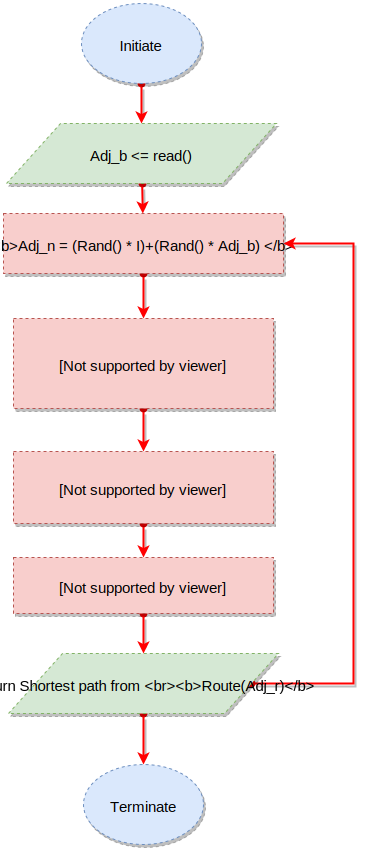
\includegraphics{reliable_routing_flow_chart.svg}

    \section{Topology computation}\label{topology-computation}

\subsection{sample topology}\label{sample-topology}

the following is a sample topology for computing.
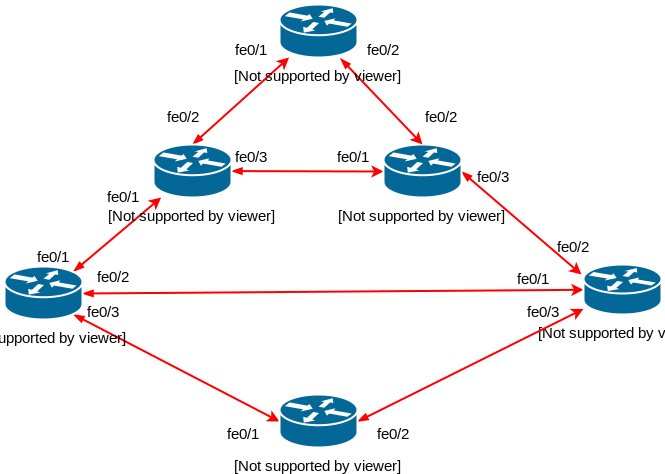
\includegraphics{initial_topo.svg}

    \subsection{Adjacency Matrix}\label{adjacency-matrix}

    \begin{Verbatim}[commandchars=\\\{\}]
{\color{incolor}In [{\color{incolor}11}]:} \PY{n}{adj} \PY{o}{=} \PY{p}{[}\PY{p}{[}\PY{l+m+mi}{0}\PY{p}{,}\PY{l+m+mi}{1}\PY{p}{,}\PY{l+m+mi}{1}\PY{p}{,}\PY{l+m+mi}{0}\PY{p}{,}\PY{l+m+mi}{0}\PY{p}{,}\PY{l+m+mi}{1}\PY{p}{]}\PY{p}{,}
                \PY{p}{[}\PY{l+m+mi}{1}\PY{p}{,}\PY{l+m+mi}{0}\PY{p}{,}\PY{l+m+mi}{0}\PY{p}{,}\PY{l+m+mi}{0}\PY{p}{,}\PY{l+m+mi}{0}\PY{p}{,}\PY{l+m+mi}{1}\PY{p}{]}\PY{p}{,}
                \PY{p}{[}\PY{l+m+mi}{1}\PY{p}{,}\PY{l+m+mi}{0}\PY{p}{,}\PY{l+m+mi}{0}\PY{p}{,}\PY{l+m+mi}{1}\PY{p}{,}\PY{l+m+mi}{1}\PY{p}{,}\PY{l+m+mi}{0}\PY{p}{]}\PY{p}{,}
                \PY{p}{[}\PY{l+m+mi}{0}\PY{p}{,}\PY{l+m+mi}{0}\PY{p}{,}\PY{l+m+mi}{1}\PY{p}{,}\PY{l+m+mi}{0}\PY{p}{,}\PY{l+m+mi}{1}\PY{p}{,}\PY{l+m+mi}{1}\PY{p}{]}\PY{p}{,}
                \PY{p}{[}\PY{l+m+mi}{0}\PY{p}{,}\PY{l+m+mi}{0}\PY{p}{,}\PY{l+m+mi}{1}\PY{p}{,}\PY{l+m+mi}{1}\PY{p}{,}\PY{l+m+mi}{0}\PY{p}{,}\PY{l+m+mi}{0}\PY{p}{]}\PY{p}{,}
                \PY{p}{[}\PY{l+m+mi}{1}\PY{p}{,}\PY{l+m+mi}{1}\PY{p}{,}\PY{l+m+mi}{0}\PY{p}{,}\PY{l+m+mi}{1}\PY{p}{,}\PY{l+m+mi}{0}\PY{p}{,}\PY{l+m+mi}{0}\PY{p}{]}\PY{p}{]}
\end{Verbatim}


    \begin{Verbatim}[commandchars=\\\{\}]
{\color{incolor}In [{\color{incolor}12}]:} \PY{k+kn}{import} \PY{n+nn}{pandas} \PY{k}{as} \PY{n+nn}{pd}
         \PY{n}{pd}\PY{o}{.}\PY{n}{DataFrame}\PY{p}{(}\PY{n}{adj}\PY{p}{)}
\end{Verbatim}


\begin{Verbatim}[commandchars=\\\{\}]
{\color{outcolor}Out[{\color{outcolor}12}]:}    0  1  2  3  4  5
         0  0  1  1  0  0  1
         1  1  0  0  0  0  1
         2  1  0  0  1  1  0
         3  0  0  1  0  1  1
         4  0  0  1  1  0  0
         5  1  1  0  1  0  0
\end{Verbatim}
            
    \begin{Verbatim}[commandchars=\\\{\}]
{\color{incolor}In [{\color{incolor}186}]:} \PY{k+kn}{import} \PY{n+nn}{networkx} \PY{k}{as} \PY{n+nn}{nx}
          \PY{k+kn}{import} \PY{n+nn}{matplotlib}\PY{n+nn}{.}\PY{n+nn}{pyplot} \PY{k}{as} \PY{n+nn}{plt}
          \PY{o}{\PYZpc{}}\PY{k}{matplotlib} inline
          
          \PY{n}{topo}\PY{o}{=}\PY{n}{nx}\PY{o}{.}\PY{n}{MultiDiGraph}\PY{p}{(}\PY{p}{)}
          
          \PY{k}{def} \PY{n+nf}{create\PYZus{}topo}\PY{p}{(}\PY{n}{graph}\PY{p}{,} \PY{n}{adj\PYZus{}matrix}\PY{p}{)}\PY{p}{:}
              \PY{k}{for} \PY{n}{i} \PY{o+ow}{in} \PY{n+nb}{range}\PY{p}{(}\PY{n+nb}{len}\PY{p}{(}\PY{n}{adj\PYZus{}matrix}\PY{p}{)}\PY{p}{)}\PY{p}{:}
                  \PY{k}{for} \PY{n}{j} \PY{o+ow}{in} \PY{n+nb}{range}\PY{p}{(}\PY{n+nb}{len}\PY{p}{(}\PY{n}{adj\PYZus{}matrix}\PY{p}{[}\PY{n}{i}\PY{p}{]}\PY{p}{)}\PY{p}{)}\PY{p}{:}
                      \PY{k}{if} \PY{n}{adj\PYZus{}matrix}\PY{p}{[}\PY{n}{i}\PY{p}{]}\PY{p}{[}\PY{n}{j}\PY{p}{]} \PY{o}{!=} \PY{l+m+mi}{0}\PY{p}{:}
                          \PY{n}{graph}\PY{o}{.}\PY{n}{add\PYZus{}edge}\PY{p}{(}\PY{l+s+s1}{\PYZsq{}}\PY{l+s+s1}{node\PYZus{}}\PY{l+s+s1}{\PYZsq{}}\PY{o}{+}\PY{n+nb}{str}\PY{p}{(}\PY{n}{i}\PY{o}{+}\PY{l+m+mi}{1}\PY{p}{)}\PY{p}{,}\PY{l+s+s1}{\PYZsq{}}\PY{l+s+s1}{node\PYZus{}}\PY{l+s+s1}{\PYZsq{}}\PY{o}{+}\PY{n+nb}{str}\PY{p}{(}\PY{n}{j}\PY{o}{+}\PY{l+m+mi}{1}\PY{p}{)}\PY{p}{)}
                          \PY{n+nb}{print}\PY{p}{(}\PY{n}{f}\PY{l+s+s1}{\PYZsq{}}\PY{l+s+s1}{node\PYZus{}}\PY{l+s+s1}{\PYZob{}}\PY{l+s+s1}{i+1\PYZcb{} , node\PYZus{}}\PY{l+s+s1}{\PYZob{}}\PY{l+s+s1}{j+1\PYZcb{} : Added}\PY{l+s+s1}{\PYZsq{}}\PY{p}{)}
              \PY{k}{return} \PY{n}{graph}
          
          \PY{n}{topo}\PY{o}{=}\PY{n}{create\PYZus{}topo}\PY{p}{(}\PY{n}{graph}\PY{o}{=}\PY{n}{topo}\PY{p}{,} \PY{n}{adj\PYZus{}matrix}\PY{o}{=}\PY{n}{adj}\PY{p}{)}
          \PY{n}{nx}\PY{o}{.}\PY{n}{draw}\PY{p}{(}\PY{n}{topo}\PY{p}{,} \PY{n}{pos}\PY{o}{=}\PY{n}{nx}\PY{o}{.}\PY{n}{spring\PYZus{}layout}\PY{p}{(}\PY{n}{topo}\PY{p}{)}\PY{p}{,} \PY{n}{with\PYZus{}labels}\PY{o}{=}\PY{k+kc}{True}\PY{p}{)}
\end{Verbatim}


    \begin{Verbatim}[commandchars=\\\{\}]
node\_1 , node\_2 : Added
node\_1 , node\_3 : Added
node\_1 , node\_6 : Added
node\_2 , node\_1 : Added
node\_2 , node\_6 : Added
node\_3 , node\_1 : Added
node\_3 , node\_4 : Added
node\_3 , node\_5 : Added
node\_4 , node\_3 : Added
node\_4 , node\_5 : Added
node\_4 , node\_6 : Added
node\_5 , node\_3 : Added
node\_5 , node\_4 : Added
node\_6 , node\_1 : Added
node\_6 , node\_2 : Added
node\_6 , node\_4 : Added

    \end{Verbatim}

    \begin{center}
    \adjustimage{max size={0.9\linewidth}{0.9\paperheight}}{output_5_1.png}
    \end{center}
    { \hspace*{\fill} \\}
    
    \subsection{Matrix Computation with
SciPy}\label{matrix-computation-with-scipy}

    \begin{Verbatim}[commandchars=\\\{\}]
{\color{incolor}In [{\color{incolor}10}]:} \PY{k+kn}{import} \PY{n+nn}{numpy} \PY{k}{as} \PY{n+nn}{np}
         \PY{k+kn}{import} \PY{n+nn}{scipy} \PY{k}{as} \PY{n+nn}{sp}
\end{Verbatim}


    \subsubsection{Creating A numpy matrix from list
structure}\label{creating-a-numpy-matrix-from-list-structure}

    \begin{Verbatim}[commandchars=\\\{\}]
{\color{incolor}In [{\color{incolor}17}]:} \PY{n}{adj\PYZus{}b}\PY{o}{=}\PY{n}{np}\PY{o}{.}\PY{n}{matrix}\PY{p}{(}\PY{n}{adj}\PY{p}{)}
         \PY{n+nb}{print}\PY{p}{(}\PY{n}{adj\PYZus{}b}\PY{p}{)}
\end{Verbatim}


    \begin{Verbatim}[commandchars=\\\{\}]
[[0 1 1 0 0 1]
 [1 0 0 0 0 1]
 [1 0 0 1 1 0]
 [0 0 1 0 1 1]
 [0 0 1 1 0 0]
 [1 1 0 1 0 0]]

    \end{Verbatim}

    \subsubsection{Creating random matrix}\label{creating-random-matrix}

    \begin{Verbatim}[commandchars=\\\{\}]
{\color{incolor}In [{\color{incolor}24}]:} \PY{n}{rand} \PY{o}{=} \PY{n}{np}\PY{o}{.}\PY{n}{random}\PY{o}{.}\PY{n}{rand}\PY{p}{(}\PY{n}{adj\PYZus{}b}\PY{o}{.}\PY{n}{shape}\PY{p}{[}\PY{l+m+mi}{0}\PY{p}{]}\PY{p}{,} \PY{n}{adj\PYZus{}b}\PY{o}{.}\PY{n}{shape}\PY{p}{[}\PY{l+m+mi}{1}\PY{p}{]}\PY{p}{)}
         \PY{n}{pd}\PY{o}{.}\PY{n}{DataFrame}\PY{p}{(}\PY{n}{rand}\PY{p}{)}
\end{Verbatim}


\begin{Verbatim}[commandchars=\\\{\}]
{\color{outcolor}Out[{\color{outcolor}24}]:}           0         1         2         3         4         5
         0  0.716932  0.769974  0.877032  0.662190  0.134626  0.491502
         1  0.373797  0.004641  0.687809  0.523381  0.214858  0.857767
         2  0.736524  0.183897  0.988929  0.152798  0.590443  0.417242
         3  0.800924  0.320144  0.529795  0.780656  0.337633  0.916752
         4  0.033966  0.794648  0.283359  0.491431  0.055972  0.024841
         5  0.605942  0.959043  0.357256  0.809237  0.946049  0.064220
\end{Verbatim}
            
    \subsubsection{\texorpdfstring{Element wise multiplicartion
\(adj_e = rand \cdot adj_b\)}{Element wise multiplicartion adj\_e = rand \textbackslash{}cdot adj\_b}}\label{element-wise-multiplicartion-adj_e-rand-cdot-adj_b}

    \begin{Verbatim}[commandchars=\\\{\}]
{\color{incolor}In [{\color{incolor}23}]:} \PY{n}{adj\PYZus{}e} \PY{o}{=} \PY{n}{np}\PY{o}{.}\PY{n}{multiply}\PY{p}{(}\PY{n}{rand}\PY{p}{,} \PY{n}{adj\PYZus{}b}\PY{p}{)}
         \PY{n}{pd}\PY{o}{.}\PY{n}{DataFrame}\PY{p}{(}\PY{n}{adj\PYZus{}e}\PY{p}{)}
\end{Verbatim}


\begin{Verbatim}[commandchars=\\\{\}]
{\color{outcolor}Out[{\color{outcolor}23}]:}           0         1         2         3         4         5
         0  0.000000  0.933323  0.863578  0.000000  0.000000  0.382751
         1  0.264790  0.000000  0.000000  0.000000  0.000000  0.480461
         2  0.042530  0.000000  0.000000  0.598267  0.221010  0.000000
         3  0.000000  0.000000  0.567996  0.000000  0.082535  0.345213
         4  0.000000  0.000000  0.078449  0.129976  0.000000  0.000000
         5  0.077746  0.821450  0.000000  0.783321  0.000000  0.000000
\end{Verbatim}
            
    \subsubsection{\texorpdfstring{Calulating
\(Adj_n = (rand \cdot I) + Adj_e\)}{Calulating Adj\_n = (rand \textbackslash{}cdot I) + Adj\_e}}\label{calulating-adj_n-rand-cdot-i-adj_e}

    \begin{Verbatim}[commandchars=\\\{\}]
{\color{incolor}In [{\color{incolor}37}]:} \PY{n}{x}\PY{o}{=}\PY{n}{np}\PY{o}{.}\PY{n}{multiply}\PY{p}{(}\PY{n}{np}\PY{o}{.}\PY{n}{random}\PY{o}{.}\PY{n}{rand}\PY{p}{(}\PY{n}{adj\PYZus{}b}\PY{o}{.}\PY{n}{shape}\PY{p}{[}\PY{l+m+mi}{0}\PY{p}{]}\PY{p}{,}\PY{n}{adj\PYZus{}b}\PY{o}{.}\PY{n}{shape}\PY{p}{[}\PY{l+m+mi}{1}\PY{p}{]}\PY{p}{)} \PY{p}{,} \PY{n}{np}\PY{o}{.}\PY{n}{identity}\PY{p}{(}\PY{n}{adj\PYZus{}b}\PY{o}{.}\PY{n}{shape}\PY{p}{[}\PY{l+m+mi}{0}\PY{p}{]}\PY{p}{)}\PY{p}{)}
         \PY{n}{pd}\PY{o}{.}\PY{n}{DataFrame}\PY{p}{(}\PY{n}{x}\PY{p}{)}
\end{Verbatim}


\begin{Verbatim}[commandchars=\\\{\}]
{\color{outcolor}Out[{\color{outcolor}37}]:}           0         1         2         3         4         5
         0  0.649591  0.000000  0.000000  0.000000  0.000000  0.000000
         1  0.000000  0.356627  0.000000  0.000000  0.000000  0.000000
         2  0.000000  0.000000  0.712613  0.000000  0.000000  0.000000
         3  0.000000  0.000000  0.000000  0.790035  0.000000  0.000000
         4  0.000000  0.000000  0.000000  0.000000  0.216337  0.000000
         5  0.000000  0.000000  0.000000  0.000000  0.000000  0.861278
\end{Verbatim}
            
    \begin{Verbatim}[commandchars=\\\{\}]
{\color{incolor}In [{\color{incolor}77}]:} \PY{n}{adj\PYZus{}n} \PY{o}{=} \PY{n}{x} \PY{o}{+} \PY{n}{adj\PYZus{}e}
         \PY{n}{pd}\PY{o}{.}\PY{n}{DataFrame}\PY{p}{(}\PY{n}{adj\PYZus{}n}\PY{p}{)}
\end{Verbatim}


\begin{Verbatim}[commandchars=\\\{\}]
{\color{outcolor}Out[{\color{outcolor}77}]:}           0         1         2         3         4         5
         0  0.649591  0.933323  0.863578  0.000000  0.000000  0.382751
         1  0.264790  0.356627  0.000000  0.000000  0.000000  0.480461
         2  0.042530  0.000000  0.712613  0.598267  0.221010  0.000000
         3  0.000000  0.000000  0.567996  0.790035  0.082535  0.345213
         4  0.000000  0.000000  0.078449  0.129976  0.216337  0.000000
         5  0.077746  0.821450  0.000000  0.783321  0.000000  0.861278
\end{Verbatim}
            
    \begin{Verbatim}[commandchars=\\\{\}]
{\color{incolor}In [{\color{incolor}144}]:} \PY{n}{topo\PYZus{}weighted} \PY{o}{=} \PY{n}{nx}\PY{o}{.}\PY{n}{MultiDiGraph}\PY{p}{(}\PY{n}{selfloop}\PY{o}{=}\PY{k+kc}{True}\PY{p}{)}
          
          \PY{k}{def} \PY{n+nf}{create\PYZus{}topo\PYZus{}with\PYZus{}weight}\PY{p}{(}\PY{n}{g}\PY{p}{,} \PY{n}{weighted\PYZus{}matrix}\PY{p}{)}\PY{p}{:}
              \PY{k}{for} \PY{n}{i} \PY{o+ow}{in} \PY{n+nb}{range}\PY{p}{(}\PY{n+nb}{len}\PY{p}{(}\PY{n}{weighted\PYZus{}matrix}\PY{p}{)}\PY{p}{)}\PY{p}{:}
                  \PY{k}{for} \PY{n}{j} \PY{o+ow}{in} \PY{n+nb}{range}\PY{p}{(}\PY{n+nb}{len}\PY{p}{(}\PY{n}{weighted\PYZus{}matrix}\PY{p}{)}\PY{p}{)}\PY{p}{:}
                      \PY{k}{if} \PY{n}{weighted\PYZus{}matrix}\PY{o}{.}\PY{n}{item}\PY{p}{(}\PY{n}{i}\PY{p}{,}\PY{n}{j}\PY{p}{)} \PY{o}{!=} \PY{l+m+mi}{0}\PY{p}{:}
                          
                          \PY{n}{val} \PY{o}{=} \PY{n+nb}{round}\PY{p}{(}\PY{n}{weighted\PYZus{}matrix}\PY{o}{.}\PY{n}{item}\PY{p}{(}\PY{n}{i}\PY{p}{,}\PY{n}{j}\PY{p}{)}\PY{p}{,}\PY{l+m+mi}{3}\PY{p}{)}
                          \PY{n}{g}\PY{o}{.}\PY{n}{add\PYZus{}edge}\PY{p}{(}\PY{l+s+s1}{\PYZsq{}}\PY{l+s+s1}{node\PYZus{}}\PY{l+s+s1}{\PYZsq{}}\PY{o}{+}\PY{n+nb}{str}\PY{p}{(}\PY{n}{i}\PY{o}{+}\PY{l+m+mi}{1}\PY{p}{)}\PY{p}{,}
                                     \PY{l+s+s1}{\PYZsq{}}\PY{l+s+s1}{node\PYZus{}}\PY{l+s+s1}{\PYZsq{}}\PY{o}{+}\PY{n+nb}{str}\PY{p}{(}\PY{n}{j}\PY{o}{+}\PY{l+m+mi}{1}\PY{p}{)}\PY{p}{,}
                                     \PY{n}{weight}\PY{o}{=}\PY{n}{val}\PY{p}{,}
                                     \PY{n}{lenghth}\PY{o}{=}\PY{n}{val}\PY{p}{)}
                          
                          \PY{n+nb}{print}\PY{p}{(}\PY{n}{f}\PY{l+s+s2}{\PYZdq{}}\PY{l+s+s2}{g.add\PYZus{}edge(}\PY{l+s+s2}{\PYZsq{}}\PY{l+s+s2}{node\PYZus{}}\PY{l+s+s2}{\PYZob{}}\PY{l+s+s2}{i+1\PYZcb{}}\PY{l+s+s2}{\PYZsq{}}\PY{l+s+s2}{ , }\PY{l+s+s2}{\PYZsq{}}\PY{l+s+s2}{node\PYZus{}}\PY{l+s+s2}{\PYZob{}}\PY{l+s+s2}{j+1\PYZcb{}}\PY{l+s+s2}{\PYZsq{}}\PY{l+s+s2}{, weight=}\PY{l+s+s2}{\PYZob{}}\PY{l+s+s2}{round(val,3)\PYZcb{})}\PY{l+s+s2}{\PYZdq{}}\PY{p}{)}
              \PY{k}{return} \PY{n}{g}
          
          \PY{n}{topo\PYZus{}weighted} \PY{o}{=} \PY{n}{create\PYZus{}topo\PYZus{}with\PYZus{}weight}\PY{p}{(}\PY{n}{topo\PYZus{}weighted}\PY{p}{,} \PY{n}{adj\PYZus{}n}\PY{p}{)}
          
          \PY{n}{nx}\PY{o}{.}\PY{n}{draw}\PY{p}{(}\PY{n}{topo\PYZus{}weighted}\PY{p}{,} 
                  \PY{n}{pos}\PY{o}{=}\PY{n}{nx}\PY{o}{.}\PY{n}{spring\PYZus{}layout}\PY{p}{(}\PY{n}{topo\PYZus{}weighted}\PY{p}{)}\PY{p}{,} 
                  \PY{n}{with\PYZus{}labels}\PY{o}{=}\PY{k+kc}{True}\PY{p}{)}
\end{Verbatim}


    \begin{Verbatim}[commandchars=\\\{\}]
g.add\_edge('node\_1' , 'node\_1', weight=0.65)
g.add\_edge('node\_1' , 'node\_2', weight=0.933)
g.add\_edge('node\_1' , 'node\_3', weight=0.864)
g.add\_edge('node\_1' , 'node\_6', weight=0.383)
g.add\_edge('node\_2' , 'node\_1', weight=0.265)
g.add\_edge('node\_2' , 'node\_2', weight=0.357)
g.add\_edge('node\_2' , 'node\_6', weight=0.48)
g.add\_edge('node\_3' , 'node\_1', weight=0.043)
g.add\_edge('node\_3' , 'node\_3', weight=0.713)
g.add\_edge('node\_3' , 'node\_4', weight=0.598)
g.add\_edge('node\_3' , 'node\_5', weight=0.221)
g.add\_edge('node\_4' , 'node\_3', weight=0.568)
g.add\_edge('node\_4' , 'node\_4', weight=0.79)
g.add\_edge('node\_4' , 'node\_5', weight=0.083)
g.add\_edge('node\_4' , 'node\_6', weight=0.345)
g.add\_edge('node\_5' , 'node\_3', weight=0.078)
g.add\_edge('node\_5' , 'node\_4', weight=0.13)
g.add\_edge('node\_5' , 'node\_5', weight=0.216)
g.add\_edge('node\_6' , 'node\_1', weight=0.078)
g.add\_edge('node\_6' , 'node\_2', weight=0.821)
g.add\_edge('node\_6' , 'node\_4', weight=0.783)
g.add\_edge('node\_6' , 'node\_6', weight=0.861)

    \end{Verbatim}

    \begin{center}
    \adjustimage{max size={0.9\linewidth}{0.9\paperheight}}{output_17_1.png}
    \end{center}
    { \hspace*{\fill} \\}
    
    \subsubsection{Generating Affinity
Matrix}\label{generating-affinity-matrix}

    \begin{Verbatim}[commandchars=\\\{\}]
{\color{incolor}In [{\color{incolor}194}]:} \PY{c+c1}{\PYZsh{} this fucntion takes a adj\PYZhy{}b and return row\PYZhy{}wise indexes of non\PYZhy{}zero numbers}
          
          \PY{k}{def} \PY{n+nf}{get\PYZus{}non\PYZus{}zero\PYZus{}index}\PY{p}{(}\PY{n}{adj}\PY{p}{)}\PY{p}{:}
              \PY{n}{ret}\PY{o}{=}\PY{p}{[}\PY{p}{]}
              \PY{k}{for} \PY{n}{i} \PY{o+ow}{in} \PY{n+nb}{range}\PY{p}{(}\PY{n}{adj}\PY{o}{.}\PY{n}{shape}\PY{p}{[}\PY{l+m+mi}{0}\PY{p}{]}\PY{p}{)}\PY{p}{:}
                  \PY{n}{row}\PY{o}{=}\PY{p}{[}\PY{p}{]}
                  \PY{k}{for} \PY{n}{j} \PY{o+ow}{in} \PY{n+nb}{range}\PY{p}{(}\PY{n}{adj}\PY{o}{.}\PY{n}{shape}\PY{p}{[}\PY{l+m+mi}{1}\PY{p}{]}\PY{p}{)}\PY{p}{:}
                      \PY{k}{if} \PY{n}{adj}\PY{o}{.}\PY{n}{item}\PY{p}{(}\PY{n}{i}\PY{p}{,}\PY{n}{j}\PY{p}{)}\PY{o}{!=}\PY{l+m+mi}{0}\PY{p}{:}
                          \PY{n}{row}\PY{o}{.}\PY{n}{append}\PY{p}{(}\PY{n}{j}\PY{p}{)}
                  \PY{n}{ret}\PY{o}{.}\PY{n}{append}\PY{p}{(}\PY{n}{row}\PY{p}{)}
              \PY{k}{return} \PY{n}{np}\PY{o}{.}\PY{n}{matrix}\PY{p}{(}\PY{n}{ret}\PY{p}{)}
          
          \PY{n}{nz\PYZus{}indx\PYZus{}mat} \PY{o}{=} \PY{n}{get\PYZus{}non\PYZus{}zero\PYZus{}index}\PY{p}{(}\PY{n}{adj\PYZus{}b}\PY{p}{)}
          \PY{n}{nz\PYZus{}indx\PYZus{}mat}
\end{Verbatim}


\begin{Verbatim}[commandchars=\\\{\}]
{\color{outcolor}Out[{\color{outcolor}194}]:} matrix([[list([1, 2, 5]), list([0, 5]), list([0, 3, 4]), list([2, 4, 5]),
                   list([2, 3]), list([0, 1, 3])]], dtype=object)
\end{Verbatim}
            
    \begin{Verbatim}[commandchars=\\\{\}]
{\color{incolor}In [{\color{incolor}191}]:} \PY{c+c1}{\PYZsh{} this fucntion distributes a random number in [0,1] range}
          \PY{l+s+sd}{\PYZsq{}\PYZsq{}\PYZsq{}}
          \PY{l+s+sd}{for each row, let there are n non zero elements }
          \PY{l+s+sd}{    generate n random number between [0,100]}
          \PY{l+s+sd}{    ith elemt of the row is i / sum(n numbers)}
          \PY{l+s+sd}{    \PYZob{}i1 / (r1 + .. + rn)\PYZcb{} + ... + \PYZob{}in /(r1 + ... + rn )\PYZcb{} = 1 }
          \PY{l+s+sd}{\PYZsq{}\PYZsq{}\PYZsq{}}
          \PY{k+kn}{import} \PY{n+nn}{random}
          
          \PY{k}{def} \PY{n+nf}{distribute\PYZus{}rand\PYZus{}over\PYZus{}nz\PYZus{}row}\PY{p}{(}\PY{n}{mat}\PY{p}{)}\PY{p}{:}
              \PY{n}{ret} \PY{o}{=} \PY{p}{[}\PY{p}{]}
              \PY{k}{for} \PY{n}{row} \PY{o+ow}{in} \PY{n+nb}{range}\PY{p}{(}\PY{n}{mat}\PY{o}{.}\PY{n}{shape}\PY{p}{[}\PY{l+m+mi}{1}\PY{p}{]}\PY{p}{)}\PY{p}{:}
                  \PY{n}{temp}\PY{o}{=}\PY{p}{[}\PY{p}{]}
                  \PY{k}{for} \PY{n}{i} \PY{o+ow}{in} \PY{n+nb}{range}\PY{p}{(}\PY{n+nb}{len}\PY{p}{(}\PY{n}{mat}\PY{o}{.}\PY{n}{item}\PY{p}{(}\PY{n}{row}\PY{p}{)}\PY{p}{)}\PY{p}{)}\PY{p}{:}
                      \PY{n}{temp}\PY{o}{.}\PY{n}{append}\PY{p}{(}\PY{n}{random}\PY{o}{.}\PY{n}{randint}\PY{p}{(}\PY{l+m+mi}{0}\PY{p}{,}\PY{l+m+mi}{100}\PY{p}{)}\PY{p}{)}
                  \PY{n}{r\PYZus{}sum}\PY{o}{=}\PY{n+nb}{sum}\PY{p}{(}\PY{n}{temp}\PY{p}{)}
                  \PY{k}{for} \PY{n}{i} \PY{o+ow}{in} \PY{n+nb}{range}\PY{p}{(}\PY{n+nb}{len}\PY{p}{(}\PY{n}{temp}\PY{p}{)}\PY{p}{)}\PY{p}{:}
                      \PY{n}{temp}\PY{p}{[}\PY{n}{i}\PY{p}{]} \PY{o}{=} \PY{n+nb}{round}\PY{p}{(}\PY{p}{(}\PY{n}{temp}\PY{p}{[}\PY{n}{i}\PY{p}{]} \PY{o}{/} \PY{n}{r\PYZus{}sum}\PY{p}{)}\PY{p}{,} \PY{l+m+mi}{3}\PY{p}{)}
                  \PY{n}{ret}\PY{o}{.}\PY{n}{append}\PY{p}{(}\PY{n}{temp}\PY{p}{)}
              \PY{k}{return} \PY{n}{ret}
          
          \PY{n}{nz\PYZus{}rand\PYZus{}mat} \PY{o}{=} \PY{n}{distribute\PYZus{}rand\PYZus{}over\PYZus{}nz\PYZus{}row}\PY{p}{(} \PY{n}{get\PYZus{}non\PYZus{}zero\PYZus{}index}\PY{p}{(}\PY{n}{adj\PYZus{}b}\PY{p}{)}\PY{p}{)}
          \PY{n}{pd}\PY{o}{.}\PY{n}{DataFrame}\PY{p}{(}\PY{n}{nz\PYZus{}rand\PYZus{}mat}\PY{p}{)}            
\end{Verbatim}


\begin{Verbatim}[commandchars=\\\{\}]
{\color{outcolor}Out[{\color{outcolor}191}]:}        0      1      2
          0  0.383  0.496  0.122
          1  0.714  0.286    NaN
          2  0.180  0.820  0.000
          3  0.387  0.369  0.244
          4  0.169  0.831    NaN
          5  0.182  0.460  0.358
\end{Verbatim}
            
    \begin{Verbatim}[commandchars=\\\{\}]
{\color{incolor}In [{\color{incolor}228}]:} \PY{k}{def} \PY{n+nf}{generate\PYZus{}affinity}\PY{p}{(}\PY{n}{nz\PYZus{}indx\PYZus{}mat} \PY{p}{,} \PY{n}{nz\PYZus{}rand\PYZus{}mat}\PY{p}{,} \PY{n}{adj\PYZus{}n}\PY{p}{)}\PY{p}{:}
              \PY{n}{ret}\PY{o}{=}\PY{p}{[}\PY{p}{]}
              \PY{k}{for} \PY{n}{i} \PY{o+ow}{in} \PY{n+nb}{range}\PY{p}{(}\PY{n}{adj\PYZus{}n}\PY{o}{.}\PY{n}{shape}\PY{p}{[}\PY{l+m+mi}{0}\PY{p}{]}\PY{p}{)}\PY{p}{:} 
                  \PY{n}{n\PYZus{}util} \PY{o}{=} \PY{n}{adj\PYZus{}n}\PY{o}{.}\PY{n}{item}\PY{p}{(}\PY{n}{i}\PY{p}{,}\PY{n}{i}\PY{p}{)}
                  \PY{n}{row}\PY{o}{=}\PY{p}{[}\PY{p}{]}
                  \PY{n}{k}\PY{o}{=}\PY{l+m+mi}{0}
                  \PY{k}{for} \PY{n}{j} \PY{o+ow}{in} \PY{n+nb}{range}\PY{p}{(}\PY{n}{adj\PYZus{}n}\PY{o}{.}\PY{n}{shape}\PY{p}{[}\PY{l+m+mi}{1}\PY{p}{]}\PY{p}{)}\PY{p}{:}
                      \PY{k}{if} \PY{n}{j} \PY{o+ow}{in} \PY{n}{nz\PYZus{}indx\PYZus{}mat}\PY{o}{.}\PY{n}{item}\PY{p}{(}\PY{n}{i}\PY{p}{)}\PY{p}{:}
                          \PY{n}{offset} \PY{o}{=} \PY{n}{nz\PYZus{}rand\PYZus{}mat}\PY{p}{[}\PY{n}{i}\PY{p}{]}\PY{p}{[}\PY{n}{k}\PY{p}{]} \PY{o}{*} \PY{n}{n\PYZus{}util}
                          \PY{n}{row}\PY{o}{.}\PY{n}{append}\PY{p}{(}\PY{n}{offset}\PY{p}{)}
                          \PY{n}{k}\PY{o}{+}\PY{o}{=}\PY{l+m+mi}{1}
                      \PY{k}{else}\PY{p}{:}
                          \PY{n}{row}\PY{o}{.}\PY{n}{append}\PY{p}{(}\PY{l+m+mi}{0}\PY{p}{)}
                  \PY{n}{row}\PY{p}{[}\PY{n}{i}\PY{p}{]}\PY{o}{=}\PY{o}{\PYZhy{}}\PY{n}{n\PYZus{}util}
                  \PY{n}{ret}\PY{o}{.}\PY{n}{append}\PY{p}{(}\PY{n}{row}\PY{p}{)}
              \PY{k}{return} \PY{n}{ret}
          
          \PY{n}{affifity\PYZus{}mat}\PY{o}{=}\PY{n}{generate\PYZus{}affinity}\PY{p}{(}\PY{n}{nz\PYZus{}indx\PYZus{}mat}\PY{p}{,} \PY{n}{nz\PYZus{}rand\PYZus{}mat}\PY{p}{,} \PY{n}{adj\PYZus{}n}\PY{p}{)}
          \PY{n}{pd}\PY{o}{.}\PY{n}{DataFrame}\PY{p}{(}\PY{n}{affifity\PYZus{}mat}\PY{p}{)}
\end{Verbatim}


\begin{Verbatim}[commandchars=\\\{\}]
{\color{outcolor}Out[{\color{outcolor}228}]:}           0         1         2         3         4         5
          0 -0.649591  0.248793  0.322197  0.000000  0.000000  0.079250
          1  0.254631 -0.356627  0.000000  0.000000  0.000000  0.101995
          2  0.128270  0.000000 -0.712613  0.584343  0.000000  0.000000
          3  0.000000  0.000000  0.305743 -0.790035  0.291523  0.192769
          4  0.000000  0.000000  0.036561  0.179776 -0.216337  0.000000
          5  0.156753  0.396188  0.000000  0.308338  0.000000 -0.861278
\end{Verbatim}
            
    \subsubsection{STEN (Stochastic Temporal Edge
Normalization)}\label{sten-stochastic-temporal-edge-normalization}

\(Adj_s = Affinity + Adj_n\)

    \begin{Verbatim}[commandchars=\\\{\}]
{\color{incolor}In [{\color{incolor}231}]:} \PY{n}{adj\PYZus{}s} \PY{o}{=} \PY{n}{affifity\PYZus{}mat} \PY{o}{+} \PY{n}{adj\PYZus{}n}
          \PY{n}{pd}\PY{o}{.}\PY{n}{DataFrame}\PY{p}{(}\PY{n}{adj\PYZus{}s}\PY{p}{)}
\end{Verbatim}


\begin{Verbatim}[commandchars=\\\{\}]
{\color{outcolor}Out[{\color{outcolor}231}]:}           0         1         2         3         4         5
          0  0.000000  1.182116  1.185775  0.000000  0.000000  0.462001
          1  0.519421  0.000000  0.000000  0.000000  0.000000  0.582456
          2  0.170800  0.000000  0.000000  1.182610  0.221010  0.000000
          3  0.000000  0.000000  0.873740  0.000000  0.374058  0.537982
          4  0.000000  0.000000  0.115010  0.309751  0.000000  0.000000
          5  0.234499  1.217638  0.000000  1.091658  0.000000  0.000000
\end{Verbatim}
            
    \begin{Verbatim}[commandchars=\\\{\}]
{\color{incolor}In [{\color{incolor}235}]:} \PY{n}{topo\PYZus{}s} \PY{o}{=} \PY{n}{nx}\PY{o}{.}\PY{n}{MultiDiGraph}\PY{p}{(}\PY{p}{)}
          \PY{n}{topo\PYZus{}s} \PY{o}{=} \PY{n}{create\PYZus{}topo\PYZus{}with\PYZus{}weight}\PY{p}{(}\PY{n}{topo\PYZus{}s}\PY{p}{,} \PY{n}{adj\PYZus{}s}\PY{p}{)}
          \PY{n}{nx}\PY{o}{.}\PY{n}{draw}\PY{p}{(}\PY{n}{topo\PYZus{}s}\PY{p}{,} \PY{n}{pos}\PY{o}{=}\PY{n}{nx}\PY{o}{.}\PY{n}{spectral\PYZus{}layout}\PY{p}{(}\PY{n}{topo\PYZus{}s}\PY{p}{)}\PY{p}{,} \PY{n}{with\PYZus{}labels}\PY{o}{=}\PY{k+kc}{True}\PY{p}{)}
\end{Verbatim}


    \begin{Verbatim}[commandchars=\\\{\}]
g.add\_edge('node\_1' , 'node\_2', weight=1.182)
g.add\_edge('node\_1' , 'node\_3', weight=1.186)
g.add\_edge('node\_1' , 'node\_6', weight=0.462)
g.add\_edge('node\_2' , 'node\_1', weight=0.519)
g.add\_edge('node\_2' , 'node\_6', weight=0.582)
g.add\_edge('node\_3' , 'node\_1', weight=0.171)
g.add\_edge('node\_3' , 'node\_4', weight=1.183)
g.add\_edge('node\_3' , 'node\_5', weight=0.221)
g.add\_edge('node\_4' , 'node\_3', weight=0.874)
g.add\_edge('node\_4' , 'node\_5', weight=0.374)
g.add\_edge('node\_4' , 'node\_6', weight=0.538)
g.add\_edge('node\_5' , 'node\_3', weight=0.115)
g.add\_edge('node\_5' , 'node\_4', weight=0.31)
g.add\_edge('node\_6' , 'node\_1', weight=0.234)
g.add\_edge('node\_6' , 'node\_2', weight=1.218)
g.add\_edge('node\_6' , 'node\_4', weight=1.092)

    \end{Verbatim}

    \begin{center}
    \adjustimage{max size={0.9\linewidth}{0.9\paperheight}}{output_24_1.png}
    \end{center}
    { \hspace*{\fill} \\}
    
    \subsection{Shortest Path Algorithm : Dijekstra's
Algo}\label{shortest-path-algorithm-dijekstras-algo}

    \begin{Verbatim}[commandchars=\\\{\}]
{\color{incolor}In [{\color{incolor}329}]:} \PY{k}{def} \PY{n+nf}{show\PYZus{}shortest\PYZus{}path}\PY{p}{(}\PY{n}{graph}\PY{p}{,} \PY{n}{src}\PY{p}{,} \PY{n}{dst}\PY{p}{)}\PY{p}{:}
              \PY{n}{path} \PY{o}{=} \PY{n}{nx}\PY{o}{.}\PY{n}{shortest\PYZus{}path}\PY{p}{(}\PY{n}{G}\PY{o}{=}\PY{n}{graph}\PY{p}{,} \PY{n}{source}\PY{o}{=}\PY{n}{src}\PY{p}{,} \PY{n}{target}\PY{o}{=}\PY{n}{dst}\PY{p}{)}
              \PY{n}{route} \PY{o}{=} \PY{n}{nx}\PY{o}{.}\PY{n}{Graph}\PY{p}{(}\PY{p}{)}
              \PY{k}{for} \PY{n}{i} \PY{o+ow}{in} \PY{n+nb}{range}\PY{p}{(}\PY{n+nb}{len}\PY{p}{(}\PY{n}{path}\PY{p}{)} \PY{o}{\PYZhy{}}\PY{l+m+mi}{1}\PY{p}{)}\PY{p}{:}
                  \PY{n}{route}\PY{o}{.}\PY{n}{add\PYZus{}edge}\PY{p}{(}\PY{n}{path}\PY{p}{[}\PY{n}{i}\PY{p}{]}\PY{p}{,}\PY{n}{path}\PY{p}{[}\PY{n}{i}\PY{o}{+}\PY{l+m+mi}{1}\PY{p}{]}\PY{p}{)}
              
              \PY{k}{return} \PY{n}{nx}\PY{o}{.}\PY{n}{draw}\PY{p}{(}\PY{n}{route}\PY{p}{,}\PY{n}{pos}\PY{o}{=}\PY{n}{nx}\PY{o}{.}\PY{n}{spring\PYZus{}layout}\PY{p}{(}\PY{n}{route}\PY{p}{)}\PY{p}{,} \PY{n}{with\PYZus{}labels}\PY{o}{=}\PY{k+kc}{True}\PY{p}{)}
\end{Verbatim}


    \begin{Verbatim}[commandchars=\\\{\}]
{\color{incolor}In [{\color{incolor}331}]:} \PY{n}{show\PYZus{}shortest\PYZus{}path}\PY{p}{(}\PY{n}{topo\PYZus{}s}\PY{p}{,}\PY{l+s+s1}{\PYZsq{}}\PY{l+s+s1}{node\PYZus{}1}\PY{l+s+s1}{\PYZsq{}}\PY{p}{,}\PY{l+s+s1}{\PYZsq{}}\PY{l+s+s1}{node\PYZus{}2}\PY{l+s+s1}{\PYZsq{}}\PY{p}{)}
\end{Verbatim}


    \begin{center}
    \adjustimage{max size={0.9\linewidth}{0.9\paperheight}}{output_27_0.png}
    \end{center}
    { \hspace*{\fill} \\}
    
    \begin{Verbatim}[commandchars=\\\{\}]
{\color{incolor}In [{\color{incolor}332}]:} \PY{n}{show\PYZus{}shortest\PYZus{}path}\PY{p}{(}\PY{n}{topo\PYZus{}s}\PY{p}{,}\PY{l+s+s1}{\PYZsq{}}\PY{l+s+s1}{node\PYZus{}1}\PY{l+s+s1}{\PYZsq{}}\PY{p}{,}\PY{l+s+s1}{\PYZsq{}}\PY{l+s+s1}{node\PYZus{}3}\PY{l+s+s1}{\PYZsq{}}\PY{p}{)}
\end{Verbatim}


    \begin{center}
    \adjustimage{max size={0.9\linewidth}{0.9\paperheight}}{output_28_0.png}
    \end{center}
    { \hspace*{\fill} \\}
    
    \begin{Verbatim}[commandchars=\\\{\}]
{\color{incolor}In [{\color{incolor}333}]:} \PY{n}{show\PYZus{}shortest\PYZus{}path}\PY{p}{(}\PY{n}{topo\PYZus{}s}\PY{p}{,}\PY{l+s+s1}{\PYZsq{}}\PY{l+s+s1}{node\PYZus{}1}\PY{l+s+s1}{\PYZsq{}}\PY{p}{,}\PY{l+s+s1}{\PYZsq{}}\PY{l+s+s1}{node\PYZus{}4}\PY{l+s+s1}{\PYZsq{}}\PY{p}{)}
\end{Verbatim}


    \begin{center}
    \adjustimage{max size={0.9\linewidth}{0.9\paperheight}}{output_29_0.png}
    \end{center}
    { \hspace*{\fill} \\}
    
    \section{Temporal Reliability}\label{temporal-reliability}

    \subsection{Terminologies}\label{terminologies}

    \begin{itemize}
\tightlist
\item
  \(buffer_t\) is the temporal bounded buffer of a constant size \(k\)
  \textgreater{} this stores varying weights of edges after
  \textbf{STEN} normalization sampled by time 
\item
  \textbf{quality} function \(Q(.)=w_m\mu + w_d\sigma\) is the quality
  function over \(buffer_t\) \textgreater{} \(\mu\) is the mean and
  \textgreater{} \(\sigma\) is the standard deviation 
\item
  \textbf{Reliability} function \(R(.)=Z(Q(.))\) gives the ranking
  factors and must be normalised, hence \(R(.)\in[0,1]\) \textgreater{}
  \(Z(.)\) is the Z-trasforation over \(Q(.)\) to scale
\end{itemize}

    \subsection{Generating a random sample space of given nodes and buffer
size}\label{generating-a-random-sample-space-of-given-nodes-and-buffer-size}

    \begin{Verbatim}[commandchars=\\\{\}]
{\color{incolor}In [{\color{incolor}305}]:} \PY{k}{def} \PY{n+nf}{generate\PYZus{}random\PYZus{}samples}\PY{p}{(}\PY{n}{node\PYZus{}count}\PY{p}{,} \PY{n}{buffer\PYZus{}size}\PY{p}{)}\PY{p}{:}
              \PY{n}{ret}\PY{o}{=}\PY{p}{[}\PY{p}{]}
              \PY{k}{for} \PY{n}{node\PYZus{}history} \PY{o+ow}{in} \PY{n+nb}{range}\PY{p}{(}\PY{n}{node\PYZus{}count}\PY{p}{)}\PY{p}{:}
                  \PY{n}{col}\PY{o}{=}\PY{p}{[}\PY{p}{]}
                  \PY{k}{for} \PY{n}{sample} \PY{o+ow}{in} \PY{n+nb}{range}\PY{p}{(}\PY{n}{buffer\PYZus{}size}\PY{p}{)}\PY{p}{:}
                      \PY{n}{x}\PY{o}{=}\PY{n}{np}\PY{o}{.}\PY{n}{random}\PY{o}{.}\PY{n}{randn}\PY{p}{(}\PY{p}{)}\PY{c+c1}{\PYZsh{}0,100)/100}
                      \PY{n}{y}\PY{o}{=}\PY{n}{np}\PY{o}{.}\PY{n}{random}\PY{o}{.}\PY{n}{randn}\PY{p}{(}\PY{p}{)}\PY{c+c1}{\PYZsh{}0,100)/100}
                      \PY{n}{z}\PY{o}{=}\PY{n}{np}\PY{o}{.}\PY{n}{random}\PY{o}{.}\PY{n}{randn}\PY{p}{(}\PY{p}{)}\PY{c+c1}{\PYZsh{}0,100)/100}
                      \PY{c+c1}{\PYZsh{} for more randomness (x+y)*z}
                      \PY{n}{col}\PY{o}{.}\PY{n}{append}\PY{p}{(}\PY{p}{(}\PY{p}{(}\PY{n}{x}\PY{o}{+}\PY{n}{y}\PY{p}{)}\PY{o}{*}\PY{n}{z}\PY{p}{)}\PY{o}{*}\PY{o}{*}\PY{l+m+mi}{2}\PY{p}{)}
                  \PY{n}{ret}\PY{o}{.}\PY{n}{append}\PY{p}{(}\PY{n}{col}\PY{p}{)}
              \PY{k}{return} \PY{n}{ret}
          
          \PY{n}{rand\PYZus{}sample}\PY{o}{=}\PY{n}{generate\PYZus{}random\PYZus{}samples}\PY{p}{(}\PY{n+nb}{len}\PY{p}{(}\PY{n}{topo\PYZus{}s}\PY{o}{.}\PY{n}{nodes}\PY{p}{)}\PY{p}{,} \PY{l+m+mi}{150}\PY{p}{)}
          \PY{n}{pd}\PY{o}{.}\PY{n}{DataFrame}\PY{p}{(}\PY{n}{rand\PYZus{}sample}\PY{p}{)}
\end{Verbatim}


\begin{Verbatim}[commandchars=\\\{\}]
{\color{outcolor}Out[{\color{outcolor}305}]:}         0         1          2         3         4         5          6    \textbackslash{}
          0  1.911484  0.221190   1.057798  0.891179  0.213358  0.899029   0.007689   
          1  0.009290  0.019238   0.073448  7.018580  0.856921  0.116917  17.305483   
          2  2.206144  0.496628   1.141671  0.237693  0.005999  0.044680   0.089235   
          3  1.522904  8.447696  10.126947  0.021239  0.024870  2.798433   0.402488   
          4  4.305143  2.429052   5.767657  0.036978  0.039400  0.437104   0.102668   
          5  0.058328  0.250819   2.979176  1.025630  0.242540  0.063693  12.619193   
          
                  7          8         9      {\ldots}          140       141       142  \textbackslash{}
          0  0.123770  19.493269  0.219998    {\ldots}     7.234249  1.694640  0.883191   
          1  4.320308   0.553627  3.849331    {\ldots}     0.005713  1.615685  0.318805   
          2  0.273766   8.931142  0.005575    {\ldots}     1.578395  2.029810  0.013150   
          3  0.982001   6.042265  0.050360    {\ldots}     0.000020  0.559340  0.047955   
          4  0.261938   0.008212  0.101374    {\ldots}     0.032395  0.580079  1.286180   
          5  0.011371   0.755100  0.236786    {\ldots}     0.005562  0.139356  0.395382   
          
                  143       144       145       146        147       148       149  
          0  2.219996  2.938250  0.000593  1.138598   0.324420  0.000600  0.107994  
          1  1.223505  3.545946  0.003585  0.107872  99.073902  0.009724  0.002050  
          2  6.400505  0.000004  0.163839  0.924199   0.112192  0.342674  0.001414  
          3  0.276408  0.647931  1.857998  0.507330   0.059817  0.211405  0.017830  
          4  0.008437  0.016984  0.000041  0.023877  14.758457  0.022771  2.074901  
          5  0.235939  5.982370  1.105289  0.248226   0.073300  0.053586  3.480323  
          
          [6 rows x 150 columns]
\end{Verbatim}
            
    \begin{Verbatim}[commandchars=\\\{\}]
{\color{incolor}In [{\color{incolor}316}]:} \PY{k}{def} \PY{n+nf}{get\PYZus{}median\PYZus{}sd}\PY{p}{(}\PY{n}{sampled\PYZus{}matrix}\PY{p}{)}\PY{p}{:}
              \PY{k+kn}{import} \PY{n+nn}{statistics} \PY{k}{as} \PY{n+nn}{stat}
              \PY{n}{median}\PY{o}{=}\PY{p}{[}\PY{p}{]}
              \PY{n}{sd}\PY{o}{=}\PY{p}{[}\PY{p}{]}
              \PY{k}{for} \PY{n}{node\PYZus{}history} \PY{o+ow}{in} \PY{n}{sampled\PYZus{}matrix}\PY{p}{:}
                  \PY{n}{median}\PY{o}{.}\PY{n}{append}\PY{p}{(}\PY{n}{stat}\PY{o}{.}\PY{n}{median}\PY{p}{(}\PY{n}{node\PYZus{}history}\PY{p}{)}\PY{p}{)}
                  \PY{n}{sd}\PY{o}{.}\PY{n}{append}\PY{p}{(}\PY{n}{stat}\PY{o}{.}\PY{n}{stdev}\PY{p}{(}\PY{n}{node\PYZus{}history}\PY{p}{)}\PY{p}{)}
              \PY{k}{return}\PY{p}{(}\PY{n}{median}\PY{p}{,}\PY{n}{sd}\PY{p}{)}
          
          \PY{n}{sample\PYZus{}median}\PY{p}{,} \PY{n}{sample\PYZus{}sd} \PY{o}{=} \PY{n}{get\PYZus{}median\PYZus{}sd}\PY{p}{(}\PY{n}{rand\PYZus{}sample}\PY{p}{)}
          
          \PY{n+nb}{print}\PY{p}{(}\PY{n}{sample\PYZus{}median}\PY{p}{)}
          \PY{n+nb}{print}\PY{p}{(}\PY{n}{sample\PYZus{}sd}\PY{p}{)}
          
          \PY{n}{plt}\PY{o}{.}\PY{n}{bar}\PY{p}{(}\PY{n}{topo\PYZus{}s}\PY{o}{.}\PY{n}{nodes}\PY{p}{,}\PY{n}{sample\PYZus{}sd}\PY{p}{,} \PY{n}{label}\PY{o}{=}\PY{l+s+s1}{\PYZsq{}}\PY{l+s+s1}{SD}\PY{l+s+s1}{\PYZsq{}}\PY{p}{,}\PY{n}{alpha}\PY{o}{=}\PY{l+m+mf}{0.6}\PY{p}{)}
          \PY{n}{plt}\PY{o}{.}\PY{n}{bar}\PY{p}{(}\PY{n}{topo\PYZus{}s}\PY{o}{.}\PY{n}{nodes}\PY{p}{,}\PY{n}{sample\PYZus{}median}\PY{p}{,} \PY{n}{label}\PY{o}{=}\PY{l+s+s1}{\PYZsq{}}\PY{l+s+s1}{median}\PY{l+s+s1}{\PYZsq{}}\PY{p}{,} \PY{n}{alpha}\PY{o}{=}\PY{l+m+mi}{1}\PY{p}{)}
          \PY{n}{plt}\PY{o}{.}\PY{n}{legend}\PY{p}{(}\PY{p}{)}
          \PY{n}{plt}\PY{o}{.}\PY{n}{tight\PYZus{}layout}\PY{p}{(}\PY{p}{)}
          \PY{n}{plt}\PY{o}{.}\PY{n}{show}\PY{p}{(}\PY{p}{)}
\end{Verbatim}


    \begin{Verbatim}[commandchars=\\\{\}]
[0.2333878435138509, 0.1933033601947504, 0.25798928531042775, 0.3026234501897005, 0.2360998639274594, 0.2953931577652012]
[5.213447987290084, 8.915762429067163, 3.919212411050744, 4.751942112301045, 4.434170620701857, 3.7672297284348852]

    \end{Verbatim}

    \begin{center}
    \adjustimage{max size={0.9\linewidth}{0.9\paperheight}}{output_35_1.png}
    \end{center}
    { \hspace*{\fill} \\}
    
    \subsubsection{Quality Caculation}\label{quality-caculation}

\(Q(X) = w_\mu\mu(X) + w_\sigma\sigma(X)\)

    \begin{Verbatim}[commandchars=\\\{\}]
{\color{incolor}In [{\color{incolor}321}]:} \PY{k}{def} \PY{n+nf}{get\PYZus{}Quality}\PY{p}{(}\PY{n}{s\PYZus{}median}\PY{p}{,} \PY{n}{s\PYZus{}sd}\PY{p}{,} \PY{n}{w1}\PY{o}{=}\PY{l+m+mf}{0.5}\PY{p}{,} \PY{n}{w2}\PY{o}{=}\PY{l+m+mf}{0.5}\PY{p}{)}\PY{p}{:}
              \PY{n}{q}\PY{o}{=}\PY{p}{[}\PY{p}{]}
              \PY{k}{for} \PY{n}{i} \PY{o+ow}{in} \PY{n+nb}{range}\PY{p}{(}\PY{n+nb}{len}\PY{p}{(}\PY{n}{s\PYZus{}median}\PY{p}{)}\PY{p}{)}\PY{p}{:}
                  \PY{n}{q}\PY{o}{.}\PY{n}{append}\PY{p}{(}\PY{n}{w1}\PY{o}{*}\PY{n}{s\PYZus{}median}\PY{p}{[}\PY{n}{i}\PY{p}{]} \PY{o}{+} \PY{n}{w2}\PY{o}{*}\PY{n}{s\PYZus{}sd}\PY{p}{[}\PY{n}{i}\PY{p}{]}\PY{p}{)}
              \PY{k}{return} \PY{n}{q}
          
          \PY{n}{q\PYZus{}vector} \PY{o}{=} \PY{n}{get\PYZus{}Quality}\PY{p}{(}\PY{n}{sample\PYZus{}median}\PY{p}{,} \PY{n}{sample\PYZus{}sd}\PY{p}{,} \PY{n}{w1}\PY{o}{=}\PY{l+m+mf}{0.4}\PY{p}{,} \PY{n}{w2}\PY{o}{=}\PY{l+m+mf}{0.6}\PY{p}{)}
          \PY{n+nb}{print}\PY{p}{(}\PY{n}{q\PYZus{}vector}\PY{p}{)}
          
          \PY{n}{plt}\PY{o}{.}\PY{n}{bar}\PY{p}{(}\PY{n}{topo\PYZus{}s}\PY{o}{.}\PY{n}{nodes}\PY{p}{,}\PY{n}{q\PYZus{}vector}\PY{p}{,} \PY{n}{label}\PY{o}{=}\PY{l+s+s1}{\PYZsq{}}\PY{l+s+s1}{Quality}\PY{l+s+s1}{\PYZsq{}}\PY{p}{,} \PY{n}{alpha}\PY{o}{=}\PY{l+m+mi}{1}\PY{p}{)}
          \PY{n}{plt}\PY{o}{.}\PY{n}{legend}\PY{p}{(}\PY{p}{)}
          \PY{n}{plt}\PY{o}{.}\PY{n}{tight\PYZus{}layout}\PY{p}{(}\PY{p}{)}
          \PY{n}{plt}\PY{o}{.}\PY{n}{show}\PY{p}{(}\PY{p}{)}
                  
\end{Verbatim}


    \begin{Verbatim}[commandchars=\\\{\}]
[3.221423929779591, 5.426778801518197, 2.4547231607546176, 2.9722146474565068, 2.7549423179920978, 2.3784951001670116]

    \end{Verbatim}

    \begin{center}
    \adjustimage{max size={0.9\linewidth}{0.9\paperheight}}{output_37_1.png}
    \end{center}
    { \hspace*{\fill} \\}
    
    \subsubsection{Reliability Calculation}\label{reliability-calculation}

\(R = Z(Q(X))\)

    \begin{Verbatim}[commandchars=\\\{\}]
{\color{incolor}In [{\color{incolor}322}]:} \PY{k}{def} \PY{n+nf}{get\PYZus{}Reliability}\PY{p}{(}\PY{n}{quality\PYZus{}vct}\PY{p}{)}\PY{p}{:}
              \PY{n}{R}\PY{o}{=}\PY{p}{[}\PY{p}{]}
              \PY{k}{for} \PY{n}{q} \PY{o+ow}{in} \PY{n}{quality\PYZus{}vct}\PY{p}{:}
                  \PY{n}{R}\PY{o}{.}\PY{n}{append}\PY{p}{(}\PY{p}{(}\PY{n}{q}\PY{o}{\PYZhy{}}\PY{n+nb}{min}\PY{p}{(}\PY{n}{quality\PYZus{}vct}\PY{p}{)}\PY{p}{)}\PY{o}{/}\PY{p}{(}\PY{n+nb}{max}\PY{p}{(}\PY{n}{quality\PYZus{}vct}\PY{p}{)}\PY{o}{\PYZhy{}}\PY{n+nb}{min}\PY{p}{(}\PY{n}{quality\PYZus{}vct}\PY{p}{)}\PY{p}{)}\PY{p}{)}
              \PY{k}{return} \PY{n}{R}
          
          \PY{n}{r\PYZus{}vector} \PY{o}{=} \PY{n}{get\PYZus{}Reliability}\PY{p}{(}\PY{n}{q\PYZus{}vector}\PY{p}{)}
          
          \PY{n}{plt}\PY{o}{.}\PY{n}{bar}\PY{p}{(}\PY{n}{topo\PYZus{}s}\PY{o}{.}\PY{n}{nodes}\PY{p}{,}\PY{n}{r\PYZus{}vector}\PY{p}{,} \PY{n}{label}\PY{o}{=}\PY{l+s+s1}{\PYZsq{}}\PY{l+s+s1}{Reliability}\PY{l+s+s1}{\PYZsq{}}\PY{p}{,} \PY{n}{alpha}\PY{o}{=}\PY{l+m+mi}{1}\PY{p}{)}
          \PY{n}{plt}\PY{o}{.}\PY{n}{legend}\PY{p}{(}\PY{p}{)}
          \PY{n}{plt}\PY{o}{.}\PY{n}{tight\PYZus{}layout}\PY{p}{(}\PY{p}{)}
          \PY{n}{plt}\PY{o}{.}\PY{n}{show}\PY{p}{(}\PY{p}{)}
\end{Verbatim}


    \begin{center}
    \adjustimage{max size={0.9\linewidth}{0.9\paperheight}}{output_39_0.png}
    \end{center}
    { \hspace*{\fill} \\}
    

    % Add a bibliography block to the postdoc
    
    
    
    \end{document}
